\documentclass{article}
\usepackage[a4paper, portrait, margin=1cm, right=1cm]{geometry}
\usepackage{fontspec}
\usepackage[fleqn]{amsmath}
\usepackage{setspace}
\usepackage{graphicx}

\graphicspath{./graphics/}
\setmainfont[Ligatures=TeX]{Linux Libertine}

\title{Информационные технологии. Лекция 02. Свойства КФС. Основные компоненты КФС.}
\author{Студент группы 2305 Макурин Александр}
\date{13 февраля 2023}

\begin{document}
\maketitle
\begin{sloppypar}
    \setstretch{1.8}

    \section{Свойства КФС}
    \subsection{Имманентные}
    Свойственны любой КФС

    Связь

    Механика

    Анализ окружающей среды

    \subsection{Трансцендентные}
    Зависят от реализации

    Перемещение

    Целевая нагрузка

    Взаимодействие с оператором

    \section{Архитектура (делиберативная/реактивная):}
    В зависимости от типа КФС меняются:
    \begin{itemize}
        \item Цель (идеальное функционирование/$e_i^t \rightarrow e_i^{t - 1}$ или стабильность после достижения идеального состояния)
        \item Критерии (есть/нет)

              $R = <r_1, ..., r_n>$ - все ресурсы системы. $r_1$ соответствует $e_1$.

              Достижение перечня задач:
              \[
                  \left\{\begin{array}{ll}
                      |TK^e| \rightarrow |TK| \\
                      cost(TK) \leq R
                  \end{array}\right.
              \]
              $TK$ — перечень всех задач, $TK^e$ — список выполненных задач,
              $cost$ — затраты.
        \item Стратегии (есть/нет)
              \[
                  \left\{\begin{array}{ll}
                      |TK^{ei}| \rightarrow |TK| \\
                      cost(TK^{ei}) \leq R^{ei}
                  \end{array}\right|
                  - \text{ каждый сам пытается достичь целей}
              \]

              Отличие между индивидуальным и групповым достижением целей:

              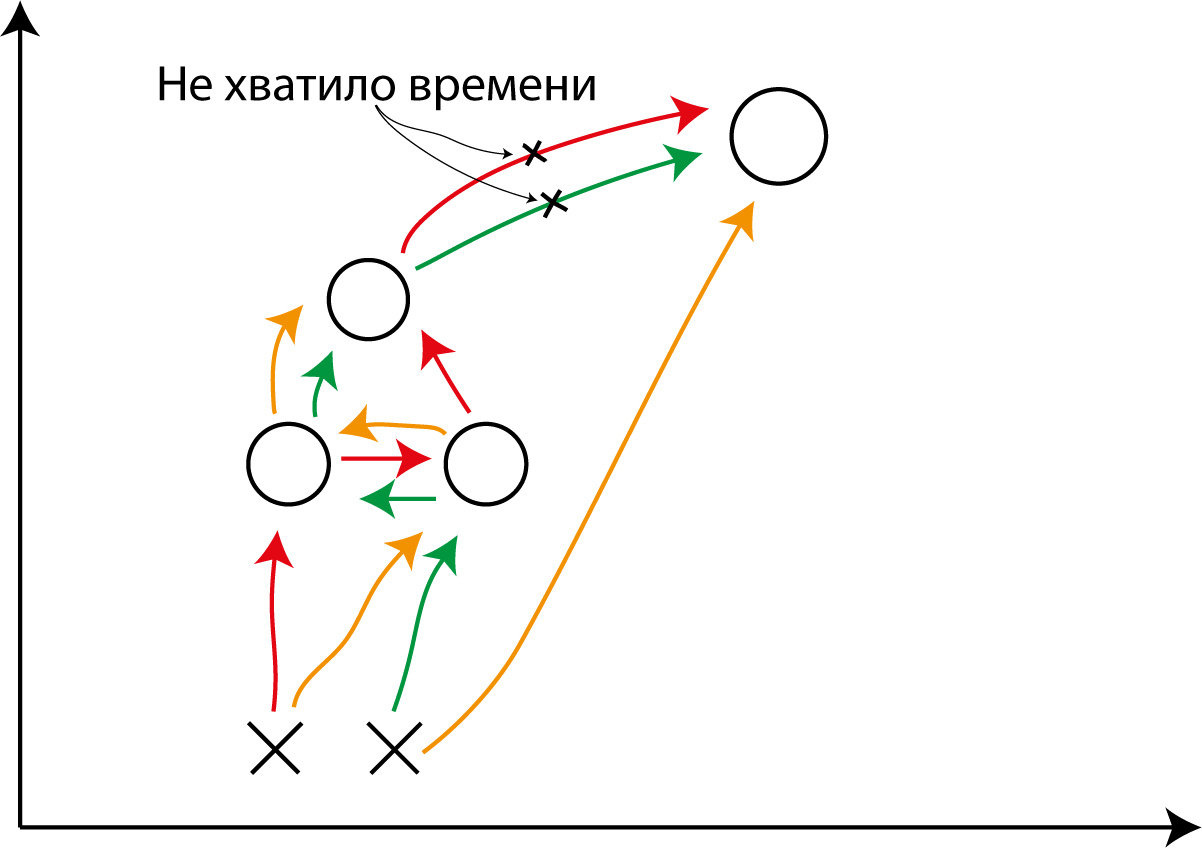
\includegraphics[width=0.6\textwidth]{graphics/Два сценария достижения цели.png}

              Круги - цели, квадраты - субъекты, стремящиеся к их достижению.
              Красные и зелёные линии обозначают случай с индивидуальной попыткой достижения целей, оранжевые - групповую попытку.

              Индивидуальное достижение цели, шаги:
              \begin{enumerate}
                  \item Субъект A движется к цели 1, субъект B движется к цели 2
                  \item Субъект A движется к цели 2, субъект B движется к цели 1
                  \item Субъекты A и B движутся к цели 3
                  \item Субъекты A и B движутся к цели 4, но у них заканчиваются
                        ресурсы и они не достигают её
              \end{enumerate}

              Групповое достижение цели:
              \begin{enumerate}
                  \item Субъект A движется к цели 1, субъект B движется к цели 4
                  \item Субъект A движется к цели 2
                  \item Субъект A движется к цели 3
                  \item Все цели достигнуты
              \end{enumerate}

        \item Взаимодействие (есть или косвенное/нет или косвенное)

              Пример — алгоритм стайного взаимодействия Boids - объекты стремятся двигаться по тому же курсу, что и соседи, при этом не сталкиваться и не отдаляться от группы.
        \item Память (есть или нет/нет) — зависит ли следующее состояние системы
              от предыдущих

              $S^{t + 1} = F(E^t, U^t, {S^{t}})$ — делиберативная c памятью \\
              $S^{t + 1} = F(E^t, U^t)$ — делиберативная \\
              $S^{t + 1} = F(U^t)$ — реактивная
    \end{itemize}

    \subsection{4 функции любой киберфизической системы:}
    \begin{itemize}
        \item Сбор информации
        \item Хранение информации
        \item Обработка информации
        \item Передача информации
    \end{itemize}

    \subsection{3 уровня связи}
    \begin{itemize}
        \item Физ $\rightarrow$ инф
        \item Инф $\rightarrow$ физ
        \item Инф $\rightarrow$ инф
    \end{itemize}

    $|W_{phy}| = const$ — мощность алфавита физических элементов системы ограничена и постоянна.

    $|W_{inf}| \rightarrow \infty$ — мощность алфавита информационных элементов системы стремится к бесконечности (в идеальной КФС).

    Канал связи принимаем условно идеальным ($P_{\text{передачи}} = 1$). Это возможно при проводной передаче на небольшие расстояния, иначе пришлось бы учитывать погрешность канала.

    Источник $\rightarrow$ канал ($\varepsilon$) $\rightarrow$ прёмник

    $B$ - пропускная способность канала

    $M$ = $U_{in_i}$ - множество сообщений

    $t_{\text{пер}} = \dfrac{M}{B}$ - время передачи

    $t_{\text{пр. р.}} = 2\alpha_1t_{\text{пер}} + \alpha_2t_{\text{формирования плана}} + \delta$, где $\delta$ - время выполнения плана, $\alpha_2$ - сложность формирования плана (зависит от оптимальности алгоритма), $\alpha_1$ - шум

    Управляемые нами параметры (на которые мы можем влиять при создании КФС):
    \begin{itemize}
        \item $B \rightarrow max$ (нас не интересует, зависит от физических параметров)
        \item $M \rightarrow min$ (нас интересует, теория кодирования)
        \item $\alpha_1 \rightarrow 1$ (нас не интересует, зависит от физических параметров)
        \item $\alpha_2 \rightarrow 0$ (нас интересует, зависит от алгоритма)
    \end{itemize}

    ЛПР (лицо принимающее решение)
    $Per : e_i \rightarrow S_{e_i}^{per}$, $Per$ — функция оценки, $e_i$ — элемент киберфизической системы, $S_{e_i}^{per}$ — субъективное представление об элементе, $S^{per}$ — пространство субъективных представлений о системе, искажение реальности.

    $S$ - пространство $\forall$ (любых) состояний системы $E$.

    В контексте КФС $\overline{S^t} = S^t + \varepsilon$, где $\overline{S^t}$ - мнение наблюдателя о системе, $S^t$ - реальное состояние $\varepsilon$ - погрешность.

    Для однозначного составления представления о системе необходимо, чтобы выполнялись следующие свойства:
    \begin{itemize}
        \item $e_i \neq e_j \Leftrightarrow Per(e_i) \neq Per(e_j)$ — если элементы КФС разные, то и их субъективное представление разное.
        \item $\forall e_i\ \exists S^{per}_{ei}$ — для каждого элемента существует соответствующее субъективное представление.
    \end{itemize}

    Свойство наблюдаемости: $\lim S_{ei}^{per} = S_{ei}$ — субъективное представление о состоянии элемента системы стремится к его реальному состоянию.

    $\Delta S \rightarrow \infty$ - мы ничего не знаем о системе.

    Варианты связи с наблюдаемостью:
    \begin{itemize}
        \item $y(t) \rightarrow 0$ - нет данных (система спит/мертва)
        \item $Per(y(t)) \rightarrow 0$ - данные есть, но наблюдатель ничего
              не понял (наблюдатель спит/мёртв)
        \item $|Per(y(t))| - |y(t)| \rightarrow 0$ — идеальный случай, наблюдатель всё понимает о каком-то элементе системе (количественное сравнение)
        \item $Per:\ \lim Per(y(t)) = Per^*$ - качественное сравнение
    \end{itemize}

    В рамках курса ЛПР=СУ (система управления).

    В контексте инф $\rightarrow$ инф:

    источник - кодировщик - канал связи (шум) - декодировщик - приёмник

    $P_{\text{приёма}} \rightarrow 0 \Leftrightarrow \text{шум} \rightarrow \infty$



\end{sloppypar}
\end{document}